\chapter{Discussion}
According to \cite{quiroz2019speeding}, a small variance of the log-likelihood ratio is crucial for a subsampling method to be successful.  

\subsection{New plots}
Here we present some plots to illustrate the differences between the different methods we presented in \textbf{the previous chapter}. 
\begin{figure}[H]
    \centering
    \includegraphics[scale = 0.7, page = 3]{figures/test.pdf}
    \caption{Caption}
    \label{fig:my_label}
\end{figure}{}

\begin{figure}[H]
    \centering
    \includegraphics[scale = 0.7, page = 4]{figures/test.pdf}
    \caption{Caption}
    \label{fig:my_label}
\end{figure}{}

\begin{figure}[H]
    \centering
    \includegraphics[scale = 0.7, page = 6]{figures/test.pdf}
    \caption{Caption}
    \label{fig:my_label}
\end{figure}{}
\section{Logistic regression}\label{sec:log_reg_experiments}







\begin{proof} From the definition of $\alpha$ and $\Tilde{\alpha}$, we have 
\begin{equation*}
\alpha - \Tilde{\alpha} = E\left[\; \mathbb{1}\left(\Lambda_N\left(\theta, \theta'\right) > \psi\left(u, \theta, \theta'\right)\right) - \mathbb{1}\left(\Lambda_T^{\star}\left(\theta, \theta'\right) > \psi\left(u, \theta, \theta'\right)\right)\right]    
\end{equation*}
which we can rewrite to
\begin{equation*}
    E\left[\; \mathbb{1}\left(\Lambda_N\left(\theta, \theta'\right) > \psi\left(u, \theta, \theta'\right)\right) - \mathbb{1}\left(\Lambda_T^{\star}\left(\theta,\theta'\right) > \psi\left(u, \theta, \theta'\right)\right)\mid T < N \right] 
\end{equation*}
since for $T = n$, $\Lambda_T^{\star}\left(\theta, \theta'\right) = \Lambda_N\left(\theta, \theta'\right)$, so  $\alpha = \Tilde{\alpha}$. We want to bound the absolute difference between $\alpha$ and $\Tilde{\alpha}$, $\mid \alpha - \Tilde{\alpha}\mid$. So we apply Jensen's inequality: 
\begin{equation}\label{eq:jensen}
\phi\left(E\left[X\right] \right) \leq E\left[\phi\left(X\right)\right] 
\end{equation}
for some convex function $\phi$. Since the absolute value, $\mid \cdot\mid$, is a convex function, we have  
\begin{equation*}
\begin{split}
\mid \alpha - \Tilde{\alpha}\mid &= 
    \mid E\left[\mathbb{1}\left(\Lambda_N\left(\theta, \theta'\right) > \psi \left(u, \theta, \theta'\right)\right) - \mathbb{1}\left(\Lambda_T^{\star}\left(\theta, \theta'\right) > \psi\left(u, \theta, \theta'\right)\right)\mid T < N\right]\mid 
    \end{split}
\end{equation*}
\begin{equation*}
    \leq E\left[\mid \mathbb{1}\left(\Lambda_N\left(\theta, \theta'\right) > \psi\left(u, \theta, \theta'\right)\right) - \mathbb{1}\left(\theta, \theta'\right) > \psi\left(u, \theta, \theta'\right)\mid T<  N\right]
\end{equation*}
If we have $\mid \mathbb{1}\left(\Lambda_N\left(\theta, \theta'\right) > \psi\left(u, \theta, \theta'\right)\right) - \mathbb{1}\left(\Lambda_T^{\star}\left(\theta, \theta'\right) > \psi\left(u, \theta, \theta'\right)\right)\mid = 1$ (\textbf{at some iteration of the Markov chain}) and using the definition of $T$ given in \eqref{eq:T_stopping} \textbf{we} see that $\mid \Lambda_n\left(\theta, \theta'\right) - \Lambda_T^{\star}\left(\theta, \theta'\right) \mid \geq c_T$, so
\begin{equation*}
\begin{split}
\mid \alpha - \Tilde{\alpha}\mid &\leq
     E\left[\mid\mathbb{1}\left(\Lambda_N\left(\theta, \theta'\right)> \psi\left(u, \theta, \theta'\right)\right) -\mathbb{1}\left( \Lambda_T^{\star}\left(\theta, \theta'\right)>\psi\left(u, \theta, \theta'\right)\right)\mid T<N \right] \\ &= E\left[\mid \mathbb{1}\left(\mid \Lambda_N\left(\theta, \theta'\right) - \Lambda_T^{\star}\left(\theta, \theta'\right)\mid \geq c_T\right)\mid T<N\right]\\ &= P\left(\mid\Lambda_N\left(\theta, \theta'\right) - \Lambda_T^{\star}\left(\theta, \theta'\right)\mid \geq c_T \mid T < N \right) \\
     & \leq P\left(\cup_{t \geq 1} \mid \Lambda_N\left(\theta, \theta'\right) - \Lambda_t^{\star}\mid \geq c_t \right) = P\left(\epsilon^c\right) = 1 - \left( 1 - \delta\right) = \delta 
\end{split}
\end{equation*}

\textbf{where the last inequality is valid since $T$ is the last of the $t$'s (by definition of $T$)}
\end{proof}